\subsubsection{A Brief History of Spreadsheets}

Although the electronic spreadsheet was first conceived in the sixties, the idea of laying out numbers in a grid dates as far back as the Babylonian times. The Plimpton 322, a Babylonian tablet from 1800 BC, lists the Pythagorean triplets in a very spreadsheet-like form, as shown in Figure \ref{fig:Plimpton}. The first two columns can be considered input and the third column represents the results of the Pythagorean calculation (which had been known years before Pythagoras was born around about 570 BC). An interesting fact about this tablet is that there is a \emph{copy-paste} error in it: one of the numbers in row 9 actually belongs in row 8. \footnote{In Section \todo{?} of this paper, we will address copy-paste errors in modern spreadsheets}

\begin{figure}
  \begin{center}
  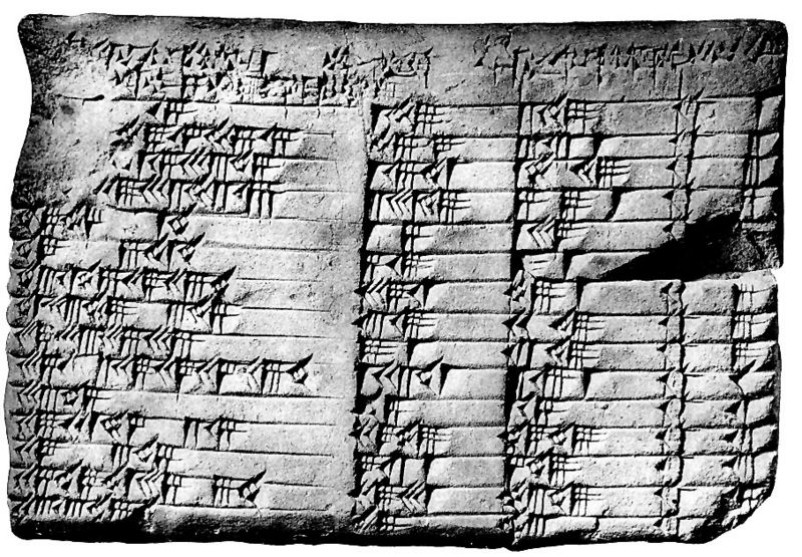
\includegraphics[width=8cm]{fig/Plimpton.png}
  \caption{Plimpton 322 showing the Pythagorean triplets: A ‘spreadsheet’ from 1800 BC}
  \label{fig:Plimpton}
  \end{center}
\end{figure} 

Mathematical tables like Plimpton 322 were used for centuries, both for mathematical purposes, such as calculation and teaching, as for administrative purposes like inventory logging. However, spreadsheet-like interfaces became more mainstream in the 15th century, when the Italian mathematician Luca Pacioli first described the double-entry bookkeeping system in his famous book `Summa de arithmetica, gemometria, proportioni et proportionalita'. This system consists of two sides: a debit and a credit side. Each transaction has to be entered twice (hence ``double-entry"), once on each side and both sides have a very spreadsheet like form. The popularity of this bookkeeping system, which is still used today in a very similar form, made the grid interface a natural representation for financial records.

The story of the electronic spreadsheet begins in 1964. In his book \emph{Simulation of the Firm through a Budget Computer Program} \cite{Mattessich1964} Mattessich ``foreshadows the basic principles behind today's computer spreadsheets: the use of matrices, (budget) simulation, and, most important, the calculation that supports each matrix cell.'' \cite{Chatfield1996}.

\begin{figure}
  \begin{center}
  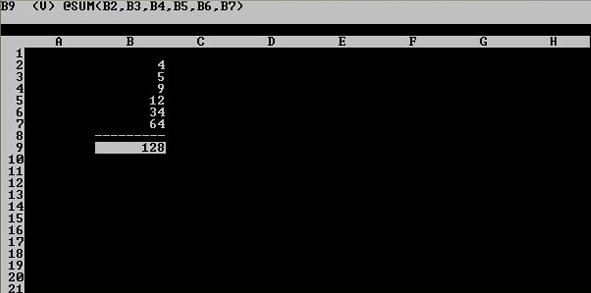
\includegraphics[width=8cm]{fig/visicalc.png}
  \caption{VisiCalc (1979)}
  \label{fig:visical}
  \end{center}
\end{figure} 


Mattessich also created 48 spreadsheets with FORTRAN IV and bundled the output with his book. The spreadsheets concerned many different domains, including ``labor costs, material costs, purchases, sales, overhead expenses with proper allocations, as well as a projected income statement and balance sheet''. These spreadsheets are generally considered the first electronic spreadsheets. 

In 1979 VisiCalc \ref{fig:visical} was created by Dan Bricklin and Bob Frankston. VisiCalc was the first commercially successful spreadsheet program, selling as much as 20.000 copies a month in 1983~\cite{Slater1989}. In many respects, VisiCalc is similar to modern spreadsheet systems. VisiCalc had the ability to automatically recalculate the value of a cell when the content was updated and to propagate this update to cells depending on it. ``This feature of automatic updating and propagation to all spreadsheet cells was so unique for a programming system that it was discussed in many books on artificial intelligence in the 1980s.'' \cite{Freedman2006}. In addition to the recalculation of cells, VisiCalc also supported copy-pasting cells and ranges with relative and absolute references. Also, it was able to construct formulas by selecting cells. 

The first version of VisiCalc ran on an Apple II. When it launched in November 1979, at a retail price of \$100, it instantly became a big hit and dealers started to bundle the software with the Apple II.\footnote{http://history-computer.com/ModernComputer/Software/Visicalc.html.} VisiCalc had a big impact on the success of the Apple II: many companies bought an Apple II solely to run VisiCalc on. As Steve Jobs himself stated in a 1994 interview with Rolling Stone magazine: ``What drove the success of the Apple II for many years and let consumers have the benefit of that product was VisiCalc selling into corporate America. Corporate America was buying Apple IIs and running VisiCalc on them like crazy." 

VisiCalc reigned the spreadsheet world until 1983, the year when Lotus 1-2-3 was released. Lotus 1-2-3 was built in highly optimized 8086 assembly-language, making it very fast. In addition to higher speed, Lotus 1-2-3 could also use more memory, which in turn allowed for larger spreadsheets. These benefits quickly made it the new industry spreadsheet standard.

In 1982 Microsoft released their first spreadsheet program: Multiplan. A fundamental difference between Multiplan and its competitors was Microsoft's decision to use R1C1 addressing instead of the A1 addressing as introduced by VisiCalc. 

Multiplan was successful on CP/M systems, but it never became as successful on MS-DOS. While Microsoft had initially planned to create a Multiplan version for Windows, this version was never released as Lotus 1-2-3 kept outselling Multiplan. Instead, Microsoft released Excel for Mac in September of 1985, just 3 years after the introduction of Multiplan. Figure \ref{fig:Excel10} shows the interface of Excel 1.0.

\begin{figure}
  \begin{center}
  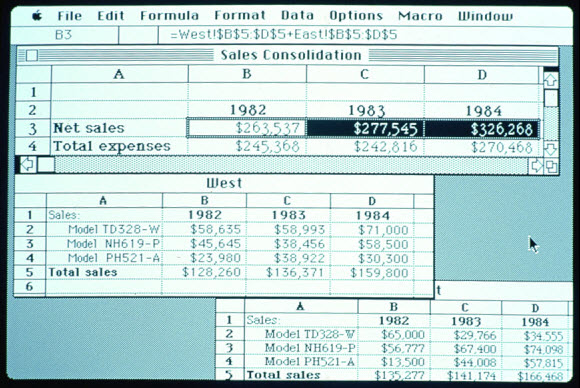
\includegraphics[width=8cm]{fig/excel10.png}
  \caption{Excel 1.0 (1985)}
  \label{fig:Excel10}
  \end{center}
\end{figure} 

One of the distinguishing features of the new Excel system was its ability to be operated with a mouse and dropdown menus. This made Excel easier and faster to use than competing spreadsheet systems. A second unique feature that contributed to Excel's popularity was the fact that users could change the style of their spreadsheets with different fonts and markup options. Finally, calculations in Excel were executed more quickly, because of optimized cell recalculation, in which only dependent cells of a modified cell are updated.

In 1987 Microsoft released Excel for Windows, and since Windows was not that popular at the time, Microsoft supplied a copy of Windows for free with each copy of Excel 2.0. Over the next few years, Excel started to challenge the position of Lotus 1-2-3. By 1988 Excel had overtaken Lotus as the dominant spreadsheet system, which it remains to date.